% Copyright 2004 by Till Tantau <tantau@users.sourceforge.net>.
%
% In principle, this file can be redistributed and/or modified under
% the terms of the GNU Public License, version 2.
%
% However, this file is supposed to be a template to be modified
% for your own needs. For this reason, if you use this file as a
% template and not specifically distribute it as part of a another
% package/program, I grant the extra permission to freely copy and
% modify this file as you see fit and even to delete this copyright
% notice. 

\documentclass{beamer}
\usepackage[utf8]{inputenc}
\usepackage[francais]{babel}

% There are many different themes available for Beamer. A comprehensive
% list with examples is given here:
% http://deic.uab.es/~iblanes/beamer_gallery/index_by_theme.html
% You can uncomment the themes below if you would like to use a different
% one:
%\usetheme{AnnArbor}
%\usetheme{Antibes}
%\usetheme{Bergen}
%\usetheme{Berkeley}
%\usetheme{Berlin}
%\usetheme{Boadilla}
%\usetheme{boxes}
%\usetheme{CambridgeUS}
%\usetheme{Copenhagen}
%\usetheme{Darmstadt}
\usetheme{default}
%\usetheme{Frankfurt}
%\usetheme{Goettingen}
%\usetheme{Hannover}
%\usetheme{Ilmenau}
%\usetheme{JuanLesPins}
%\usetheme{Luebeck}
%\usetheme{Madrid}
%\usetheme{Malmoe}
%\usetheme{Marburg}
%\usetheme{Montpellier}
%\usetheme{PaloAlto}
%\usetheme{Pittsburgh}
%\usetheme{Rochester}
%\usetheme{Singapore}
%\usetheme{Szeged}
%\usetheme{Warsaw}

\addtobeamertemplate{navigation symbols}{}{%
    \usebeamerfont{footline}%
    \usebeamercolor[fg]{footline}%
    \hspace{1em}%
    \insertframenumber%/\inserttotalframenumber
}




\title{Simulation d'un ampli EDFA en C}

\subtitle{Projet d'informatique}

\author{Jérémy Saucourt \and Gaëtan Jargot}


\date{Vendredi 24 avril 2015}

\subject{Informatique}


%\AtBeginSubsection[]
%{
%  \begin{frame}<beamer>{Table des matières}
%    \tableofcontents[currentsection,currentsubsection]
%  \end{frame}
%}

\graphicspath{{images/}}

% Let's get started
\begin{document}

{
\usebackgroundtemplate{\includegraphics[width=\paperwidth, height=\paperheight]{fibre-optique.png}}
\begin{frame}
  \titlepage
\end{frame}
}


\begin{frame}{Table des matières}
  \tableofcontents
\end{frame}


\section{Contexte et objectifs}
\begin{frame}{Contexte et objectifs}{Télécommunications optique haut débit}
  
  \begin{itemize}
  \item Télécoms optiques transocéaniques
  \item 3\textsuperscript{ème} fenêtre télécom @ 1550 nm $\rightarrow$ $A_{SiO_{2}} = 0.2~dB/km$
  \item[$\hookrightarrow$] Régénérateurs de signaux $\rightarrow$ Amplificateurs EDFA
  \item SNR limite la distance
  \end{itemize}
  
  \begin{itemize}
  \item Simulation d'un l'amplificateur EDFA en C
  \end{itemize}
  
\end{frame}




\section{Programme}

\subsection{Configuration initiale}

\begin{frame}{Configuration initiale}{}
  
  \begin{columns}[c]
  \begin{column}{.5\paperwidth}
    \includegraphics[width=.49\paperwidth]{schema_fibre.pdf}
  \end{column}
  \begin{column}{.5\paperwidth}
    \includegraphics[width=.49\paperwidth]{schema_puiss.pdf}
  \end{column}
\end{columns}
  
  \vspace{0.5cm}
  \begin{itemize}
  \item Fibre à saut d'indice
  \item Monomode pour $\lambda \in [980 ,1600]$ nm ~~($V<2.405$)
  \item C\oe ur entier dopé
  \end{itemize}
  
\end{frame}

\subsection{Algorithme}


\begin{frame}{Algorithme (Schéma)}

\begin{figure}
    \centering
    \includegraphics[width=\textwidth,height=8cm]{algo.pdf}
\end{figure}

\end{frame}

\section{Résultats}

\subsection{Courbes obtenues / Interprétation physique}

\begin{frame}{Inversion de population et puissance de pompe}
\vspace{-1cm}
\begin{figure}
    \centering
    \includegraphics[width=\textwidth,height=4cm]{N.pdf}
\end{figure}
\vspace{-1cm}
\begin{figure}
    \centering
    \includegraphics[width=\textwidth,height=4cm]{Pp.pdf}
\end{figure}

\end{frame}

\begin{frame}{Sections efficaces}

\begin{figure}
    \centering
    \includegraphics[width=\textwidth]{sigma.pdf}
\end{figure}

\end{frame}

\begin{frame}{Ps ($z$ variable)}

\begin{figure}
    \centering
    \includegraphics[width=\textwidth]{Ps.pdf}
\end{figure}

\end{frame}

\begin{frame}{Ps + $P_{ASE+}$ ($z$ variable)}

\only<1>{
\begin{figure}
    \centering
    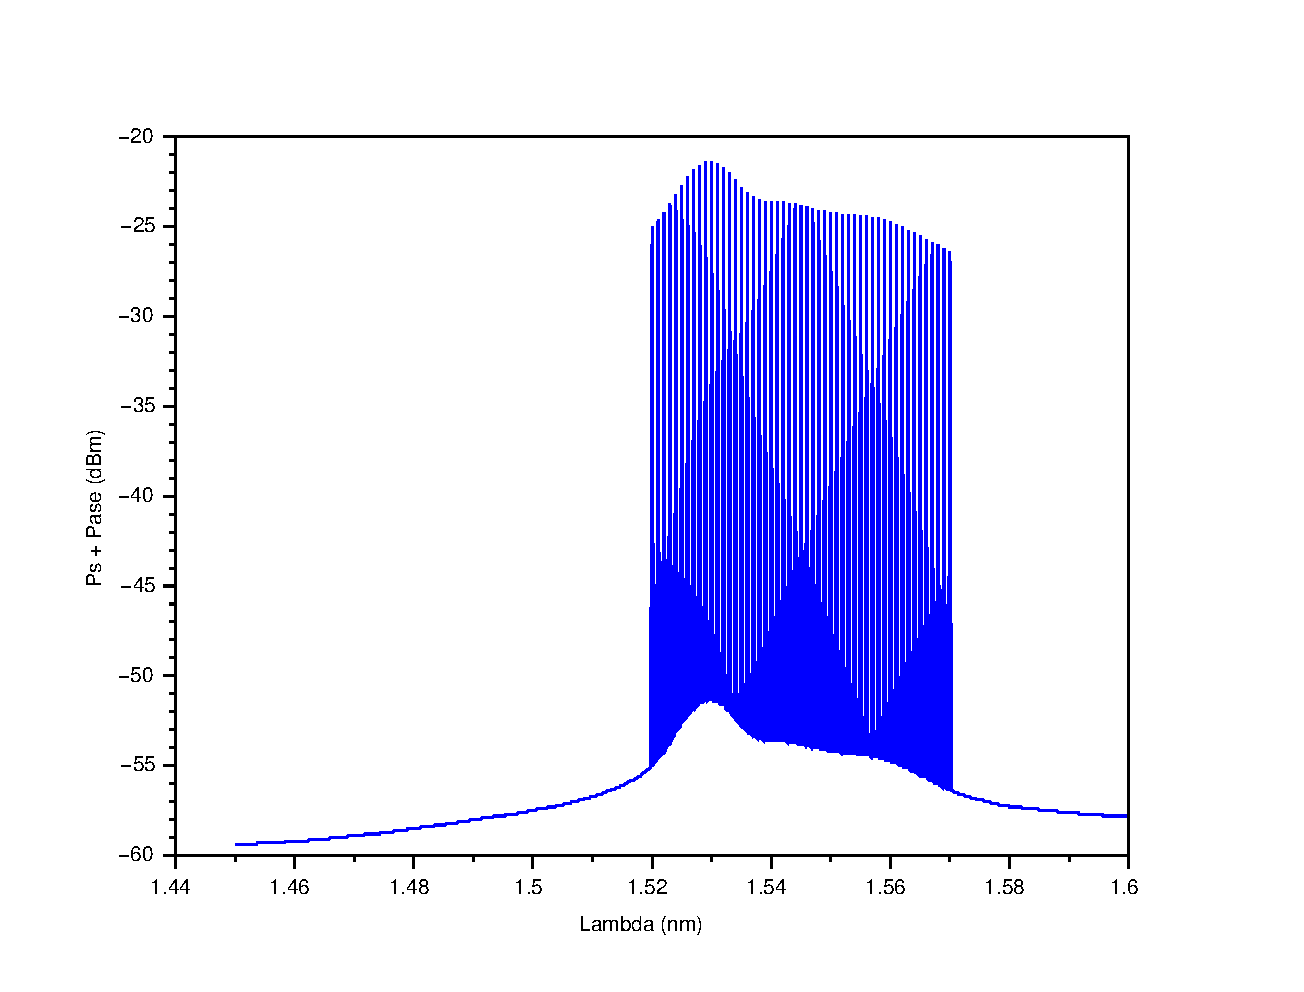
\includegraphics[width=.9\textwidth]{1m.eps}
    \caption{$z=1~m$}
\end{figure}
}

\only<2>{
\begin{figure}
    \centering
    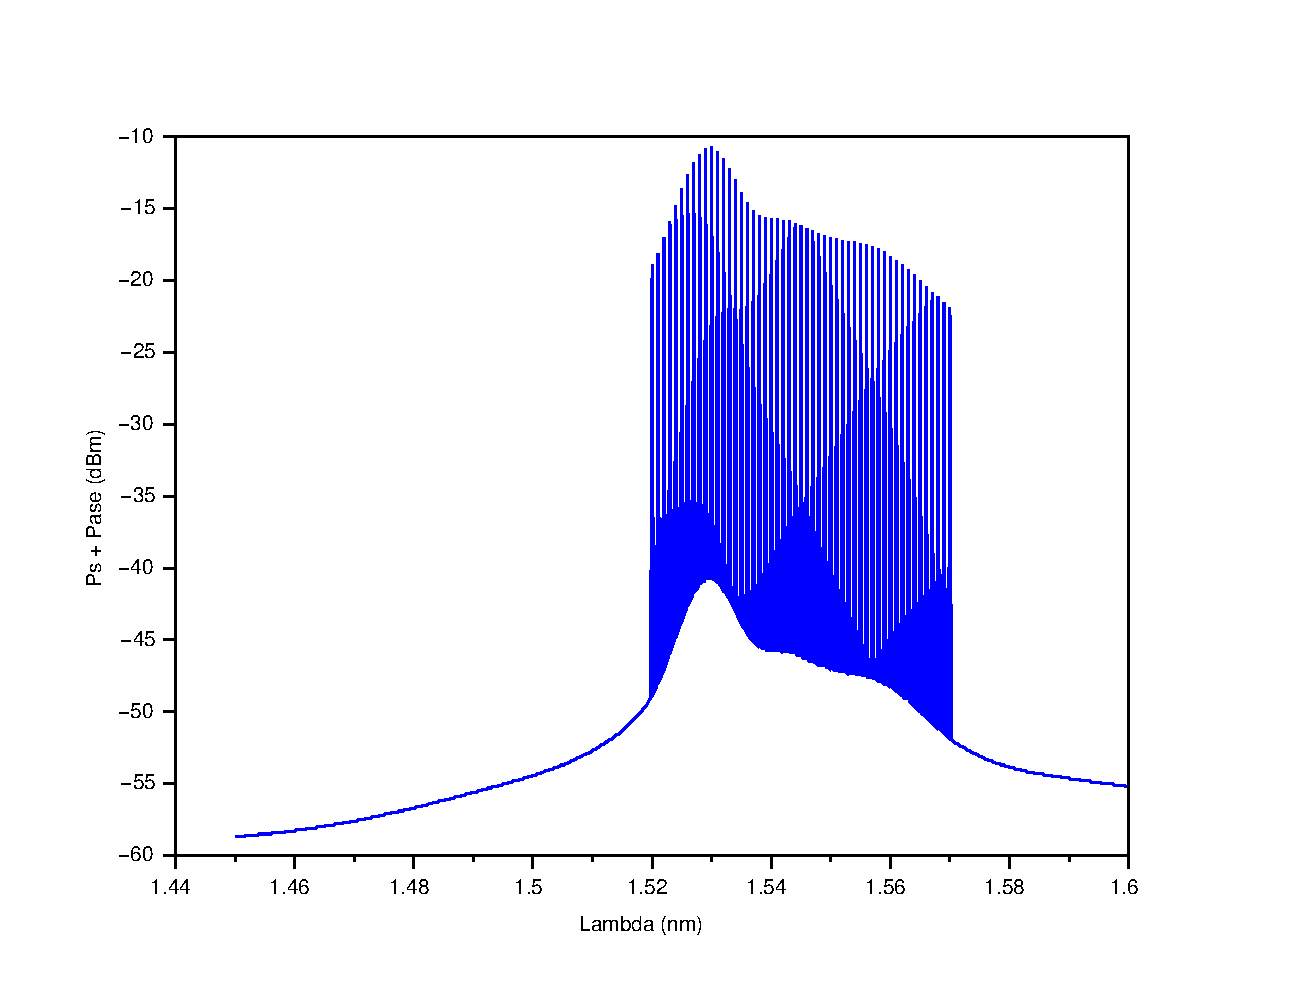
\includegraphics[width=.9\textwidth]{2m.eps}
    \caption{$z=2~m$}
\end{figure}
}

\only<3>{
\begin{figure}
    \centering
    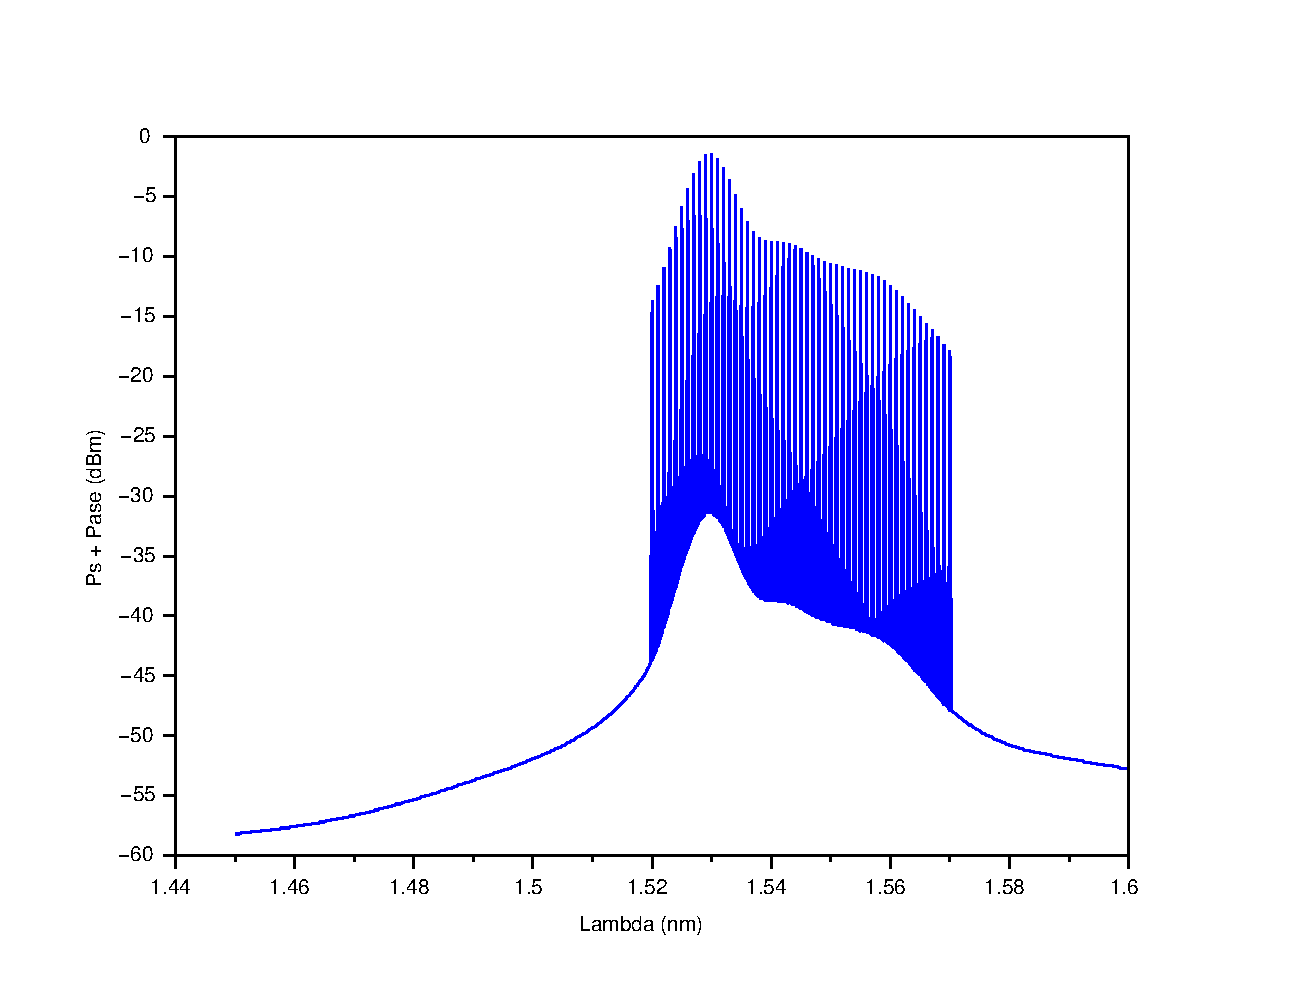
\includegraphics[width=.9\textwidth]{3m.eps}
    \caption{$z=3~m$}
\end{figure}
}

\only<4>{
\begin{figure}
    \centering
    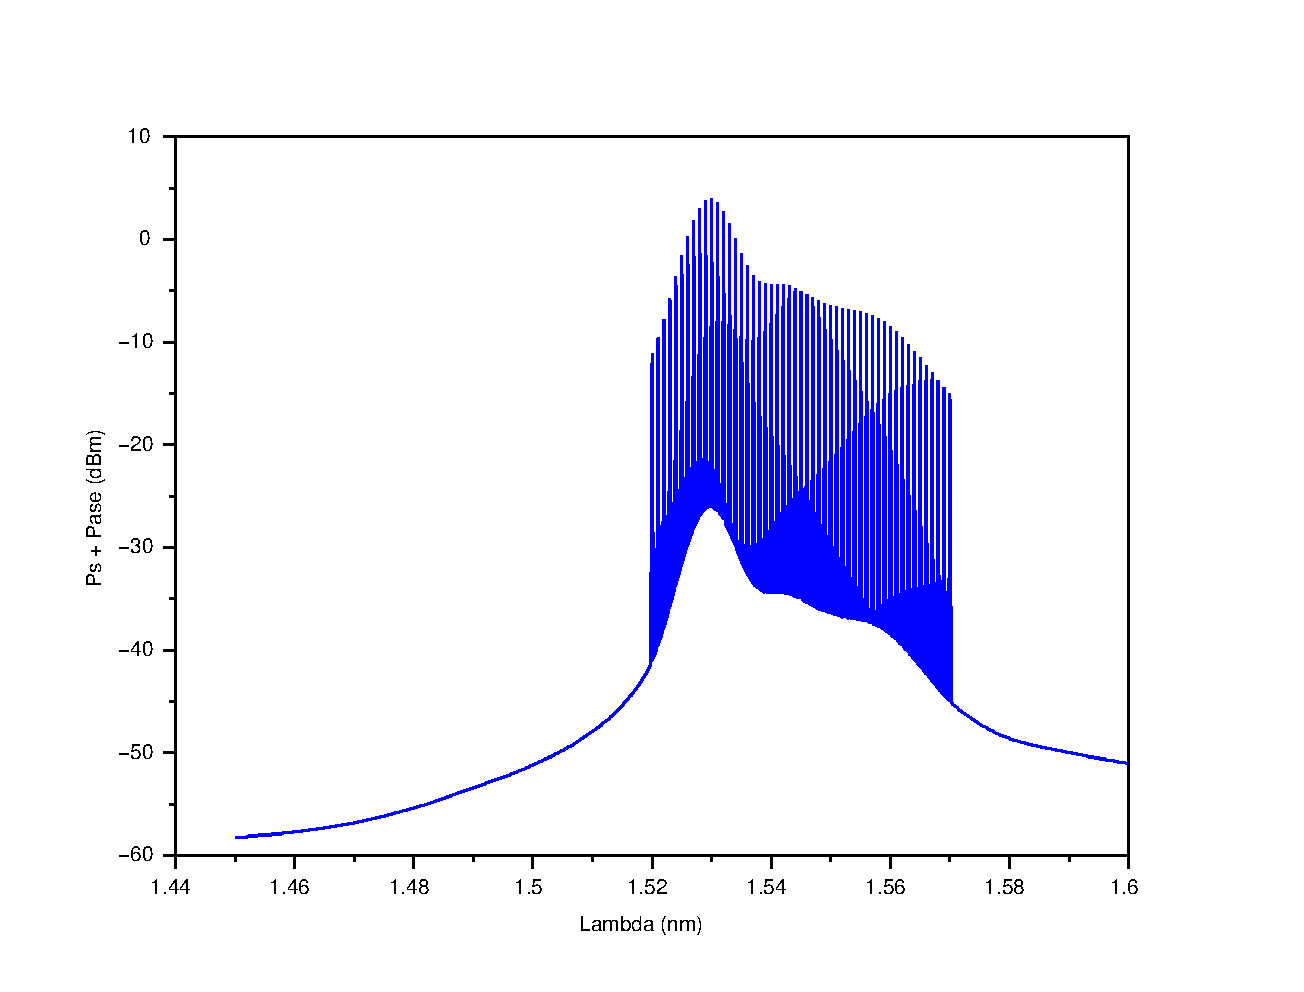
\includegraphics[width=.9\textwidth]{4m.eps}
    \caption{$z=4~m$}
\end{figure}
}

\only<5>{
\begin{figure}
    \centering
    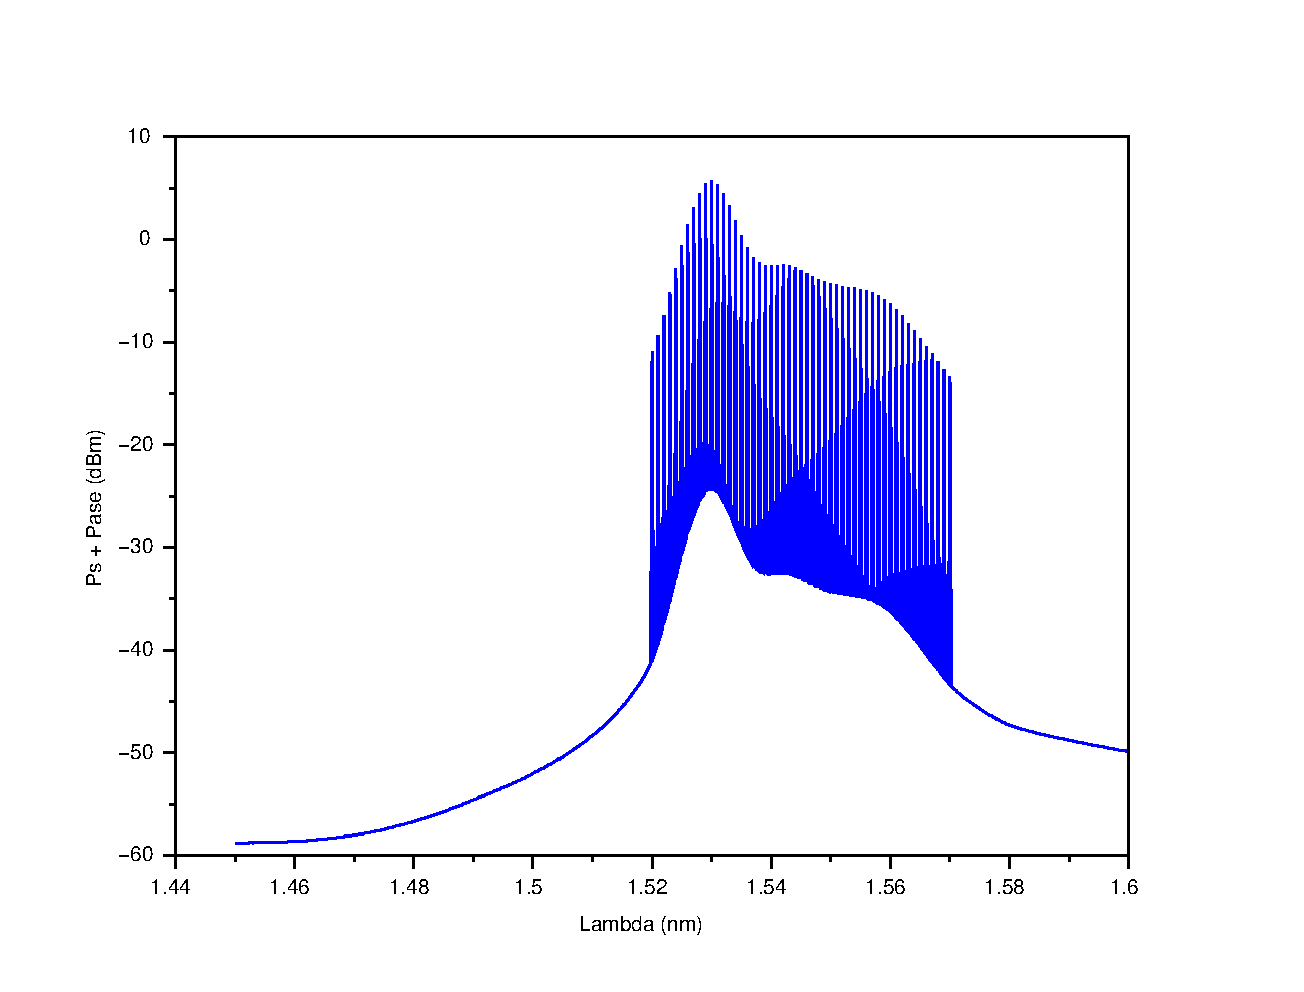
\includegraphics[width=.9\textwidth]{5m.eps}
    \caption{$z=5~m$}
\end{figure}
} 

\end{frame}


\begin{frame}{Bruit d'ASE+ ($z$ variable)}

\begin{figure}
    \centering
    \includegraphics[width=\textwidth]{bruit.pdf}
\end{figure}

\end{frame}


\begin{frame}{Résultats à 5m}{Entre 1520 nm et 1570 nm}


\begin{figure}
\centering
\begin{tabular}{|c||c|c|c|}
\hline
  & Min & Max & Valeur\\
 \hline
  $P_s$ / dBm & -13 & 6 & -\\
 \hline
 G / dB & 17 & 36 & - \\
 \hline
 SNR / dB & - & - & 11 \\
 \hline
 Ondulation / dB & - & - & 19\\
 \hline
\end{tabular}
\end{figure}




\end{frame}


\section{Conclusion et perspectives}

\begin{frame}{Conclusion et perspectives}

  \begin{itemize}
  \item Programmation en C (complexité progressive)
  \item[$\hookrightarrow$] Bonne approximation d'un EDFA ($P_{ASE-}$ négligé)
  \end{itemize}
  
  \begin{itemize}
  \item[$\leadsto$] $\nearrow$ $P_s$, en $\nearrow$ $N_0$ et $P_p$
  \item[$\leadsto$] Transformation en laser à 5 m, prise en compte des allers-retours
  \end{itemize}

\end{frame}

\end{document}

